
\documentclass[../Thesis.tex]{subfiles}
\graphicspath{{\subfix{../graphics/}}}


\begin{document}




\chapter{Quantum Computing Design Principles}

\section{Overview}
Quantum computers are capable of solving certain problems with vastly improved efficiency over their classical counterparts, as demonstrated by hallmark quantum algorithms such as Shor's factoring algorithm\cite{shor_polynomial-time_1997} and Grover's search algorithm\cite{grover_fast_1996}. %Quantum processes may also exceed classical performance at solving linear systems of equations, providing enormous advantage in a vast range of disciplines\cite{harrow_quantum_2009}. 
More recent algorithms such as the Quantum Approximation Optimization Algorithm (QAOA) or the Variational Quantum Eigensolver (VQE) leverage the power of quantum processing to find the optimal solution to a large range of problems, with potential applications to various fields, including economics, climate science, and machine learning\cite{farhi_quantum_2014}. Quantum computers are, perhaps unsurprisingly, also very well suited to the task of simulating quantum mechanical systems, and may have near term applicability to pharmaceutical development involving quantum-chemical simulations.\cite{preskill_quantum_2021,lloyd_universal_1996}.  %and allow us to probe the fundamental nature of such systems.

The qubit is the base unit of quantum information, and the building block of the quantum computer. A qubit refers to an arbitrary two-state quantum system. When discussing classical bits, it is generally assumed that these classical bits will be manifested as transistors, which have long since proven the best system we have available for classical computation. For qubits, it remains an open question which quantum system can be most effectively harnessed for computation, with various architectures being pioneered by different research groups and companies around the world.  The largest quantum processors achieved thus far are made from superconducting transmon qubits\cite{krantz_quantum_2019}, with devices exceeding 100 qubits\cite{ball_first_2021}. This is a tremendous feat of engineering, but there is a long road ahead, with conservative estimates on the number of qubits required to achieve quantum supremacy on prime factorisation starting from around 20 million\cite{gidney_how_2021}, although nearer term devices will likely prove useful for quantum-mechanical simulations\cite{childs_toward_2018}. Other leading candidates for scalable quantum computing architectures are based on photonic systems,\cite{slussarenko_photonic_2019}, ion traps\cite{bruzewicz_trapped-ion_2019}, and nuclear and electron spins\cite{vandersypen_interfacing_2017}, and as yet designing a scalable, fault-tolerant device remains an elusive goal.

%Owing to its quantum nature, the qubit can exist in a superposition of its two states.... could always save this for the later bit..

%Like the classical bit, the qubit is a two state system. However, since qubits obey the laws of quantum mechanics, they can also exist in a superposition of their two states\cite{griffiths_introduction_2005}. The difference between classical bits and qubits lies in the physics required to describe their behaviour. Classical bits, which are implemented as transistors, operate on a scale at which quantum effects average out into behaviour which is best described classically. Qubits, on the other hand, must by definition be implemented as systems whose behaviour requires a quantum mechanical description. Many quantum systems are the focus of current research seeking to achieve a scalable qubit design.



This work focuses on spin qubit devices based on phosphorus donors in silicon. Qubit arrangements in the silicon lattice are considered based on established quantum error correction codes, with a focus on IBM's recent heavy hexagon surface code\cite{chamberland_topological_2020}. Principles of quantum control are applied to designing pulses which perform desired gates between neighbouring qubit pairs, with consideration of the ramifications of current design limitations, namely the placement precision of phosphorus atoms in the silicon substrate\cite{pla_single-atom_2012}. In this chapter, an outline is provided of the key principles which form the basis of the remainder of this thesis.

\section{Quantum computing formalism}

The capability of the quantum computer to vastly outperform the classical computer is owed to two quantum mechanical phenomena: superposition, and entanglement. Superposition allows a qubit to exist in a superposition of its two states. Entanglement takes this a step further, making it possible for a system of $n$ qubits to exist in a superposition of the entire $2^n$ available states. 

The state of a single qubit can be written as
\begin{align}
    \ket{\psi} = \alpha_0\ket{0}+\alpha_1\ket{1},\ \alpha,\beta\in\mathbb{C}.
\end{align}
where 
\begin{align}
    \ket{0} = \begin{pmatrix}1 \\ 0\end{pmatrix},\quad \ket{1} = \begin{pmatrix}0 \\ 1\end{pmatrix}
\end{align}
are the basis states. 
On measurement, the qubit collapses to the $\ket{0}$ state with probability $|\alpha|^2$, or the $\ket{1}$ state with probability $|\beta|^2$. It is usual to express the qubit state in terms of angles $\theta,\phi$ as
\begin{align}
    \ket{\psi} = \cos\left(\frac{\theta}{2}\right)\ket{0} + e^{i\phi}\sin\left(\frac{\theta}{2}\right)\ket{1},\ \theta\in [0,\pi],\ \phi\in [0,2\pi).
\end{align}
The state of the qubit can thus be represented as a point on the surface of a sphere, referred to as the `Bloch sphere'. 

A system of $n$ qubits forms a register, which just like a classical register has access to $2^n$ different binary states. While superposition makes it possible for a single qubit to exist between its two states, entanglement takes this a step further, allowing the $n$-qubit state to occupy a superposition of all $2^n$ states,
\begin{align}
    \ket{\psi} = \sum_{i=0}^{N-1} \alpha_i\ket{i},\ \alpha_i\in\mathbb{C}: \Sigma_i|\alpha_i|^2=1,
\end{align}
where $N=2^n$ is the dimension of the Hilbert space of the $n$-qubit system, and the decimal $i$ in the ket is understood to represent the corresponding binary value on the $n$-qubit register.

Gates acting on an $n$-qubit system take the form of $N\times N$ matrices. Rotations of $\pi$ radians about the $x,y,z$ axes are described by the Pauli matrices,
\begin{align}
    \sigma_x = \begin{pmatrix} 0 &1\\ 1 &0\end{pmatrix},\quad 
    \sigma_y = \begin{pmatrix} 0 &-i\\ i &0\end{pmatrix},\quad
    \sigma_z = \begin{pmatrix} 1 &0\\ 0 &-1\end{pmatrix},\quad
\end{align}

Two qubit gate
\begin{align}
    \text{CNOT} = \begin{pmatrix} 1 &0 &0 &0\\ 0 &1 &0 &0\\
                            0 &0 &0 &1\\ 0 &0 &1 &0\end{pmatrix},\quad 
    \text{SWAP} = 
        \begin{pmatrix}
            1 &0 &0 &0\\
            0 &0 &1 &0\\
            0 &1 &0 &0\\
            0 &0 &0 &1
        \end{pmatrix}
\end{align}     


\section{Quantum Error Correction}
\subsection{Fault Tolerant Quantum Computing}

The quantum scale of qubits makes them hypersensitive to environmental noise, rendering their information storage inherently fragile and prone to error. This poses a formidable challenge for quantum computers to be able to withstand errors long enough to perform useful tasks. Quantum error correction codes provide a means to overcome high error rates by encoding a single logical qubit onto an array of physical qubits, and performing carefully chosen stabilizer measurements using ancilla qubits, which can indicate the presence of errors without collapsing the logical state. This resilience to noise paired with the existence of fault-tolerant gates which can be applied on the logical state space may yet allow us to achieve fault tolerant quantum computing\cite{nielsen_quantum_2010}. As such, quantum error correction is of key importance in the development of operational quantum computers.

A particularly promising family of error correction codes are surface codes,\cite{fowler_surface_2012} in which qubits are arrayed on a 2D plane, with each data qubit surrounded by ancillas which check it for errors. This design naturally lends itself to physical implementation, where close proximity of ancilla qubits to the data qubits for whose syndrome measurements they are responsible is a necessity in most quantum computing architectures. Also of relevance to this work is the Bacon-Shor subsystem code\cite{bacon_quantum_2006}, a reformulation of Shor's original stabilizer code published in 1995\cite{shor_scheme_1995}, in which logical qubits utilize 9 physical qubits to protect against both phase-flip and bit-flip errors.

\subsection{Formalism}
The group theoretical description of quantum error correction will now be introduced in the context of the 3-bit repetition code for correcting bit-flip errors. 
Quantum error correction works by encoding the state of a qubit onto many qubits. 
These qubits are called data qubits, and their state will be denoted $\ket{\Phi}$. The single qubit state which they are trying to preserve is called a logical qubit, identified with an $L$ subscript, $\ket{\psi}_L$. The purpose of the encoding is so that errors on the data qubits will no longer cause the logical state to be lost, although a sufficient number of errors will be able to overwhelm the error correction scheme. For the 3-bit repetition code, the logical states are encoded as
\begin{align}
    \ket{0}_L=\ket{000},\quad \ket{1}_L=\ket{111},
\end{align}
and it can be seen that if one of the data qubits were to flip its state, we would still be able to obtain the correct logical state measurement based of the majority vote of the three data qubits.


In order for errors in the data qubits to be detected, measurements of the correlations between certain data qubits are made. The operators which measure these correlations are comprised of tensor products of Pauli matrices. For the 3-bit repetition code, the operators $Z_1Z_2$ are used to measure the correlation between the spins of data qubits 1 and 2. $\langle Z_1Z_2\rangle = 1 (-1)$ would inform us that the two qubits are in the same (opposite) state. Table \ref{tab:3-bit-rep} indicates the location of bit-flip errors corresponding to each stabilizer measurement outcome.
\begin{table}[]
    \centering
    \begin{tabular}{ccc}
        \hline
         \langle Z_1Z_2\rangle &\langle Z_2Z_3\rangle&Error  \\\hline 
          0 &0 &None \\
         0 &1 &qubit 3\\
         1 &0 &qubit 1\\
         1 &1 &qubit 2\\\hline
    \end{tabular}
    \caption{Errors indicated by each possible outcome of stabilizer measurements on 3-bit X-error correcting code.}
    \label{tab:3-bit-rep}
\end{table}
The set of all possible tensor products of Pauli matrices acting on an $n$ qubit Hilbert space form a group called the Pauli group, denoted $\mathcal{P}_n$. In general, the set of stabilizers form an abelian subgroup $\mathcal{S}\leq \mathcal{P}_n$\footnote{An abelian group is a group whose elements commute with each other.}. Each stabilizer element $S\in\mathcal{S}$ acts on the Hilbert space of the data qubits, and the eigenspace of $\mathcal{S}$ is denoted $\mathcal{H}_S$, noting that each $S$ in $\mathcal{S}$ shares the same eigenspace since $\mathcal{S}$ is abelian. In the case of the 3-bit repetition code, this translates to
\begin{align}
    \mathcal{S} = \langle Z_1Z_2, Z_2Z_3\rangle,\quad \mathcal{H}_S = \left\{\ket{000},\ket{001},\dots,\ket{110},\ket{111}\right\}.
\end{align}
The eigenvalues of each state in $\mathcal{H}_S$ are all either $+1$ or $-1$. The eigenstates having eigenvalue $+1$ are precisely the logical qubit states, 
\begin{align}
    \mathcal{H}_L=\left\{\ket{0}_L,\ket{1}_L\right\},
\end{align}
while the remaining states with eigenvalue $-1$ will only be occupied when an error has occurred. For the 3-bit repeitition code,
\begin{align}
    \mathcal{H}_L = \{\ket{000},\ket{111}\}
\end{align}

\subsection{Surface codes}

Surface codes involve arrangements of qubits on a 2-dimensional grid, with ancilla qubits interspersed between data qubits whose correlations they are to measure. Surface codes are perhaps the most promising family of quantum error correction codes, requiring only nearest neighbour coupling and thus naturally lending themselves to implementation on physical devices, as well as boasting higher error thresholds than other well studied error correction protocols such as the Steane or Bacon-Shor codes\cite{fowler_surface_2012}. 
The locations of data qubits on a square surface code can be described by coordinates $(m,n)$. The stabilizers are then take the form 
\begin{align}
    \mathcal{S} = \langle Z_{m,n}Z_{m,n+1}Z_{m+1,n+1}Z_{m+1,n},\  X_{m,n}X_{m,n+1}X_{m+1,n+1}X_{m+1,n}\rangle_{mn}
\end{align}
Stabilizer routines shown in figure \ref{fig:surface} are used to obtain stabilizer measurements. Measurements of $\ket{1}$ on ancilla qubits indicate the presence of errors, and  the locations of the ancillas qubits on which these errors are registered can be used to identify the location of the error.

\begin{figure}
    \centering
    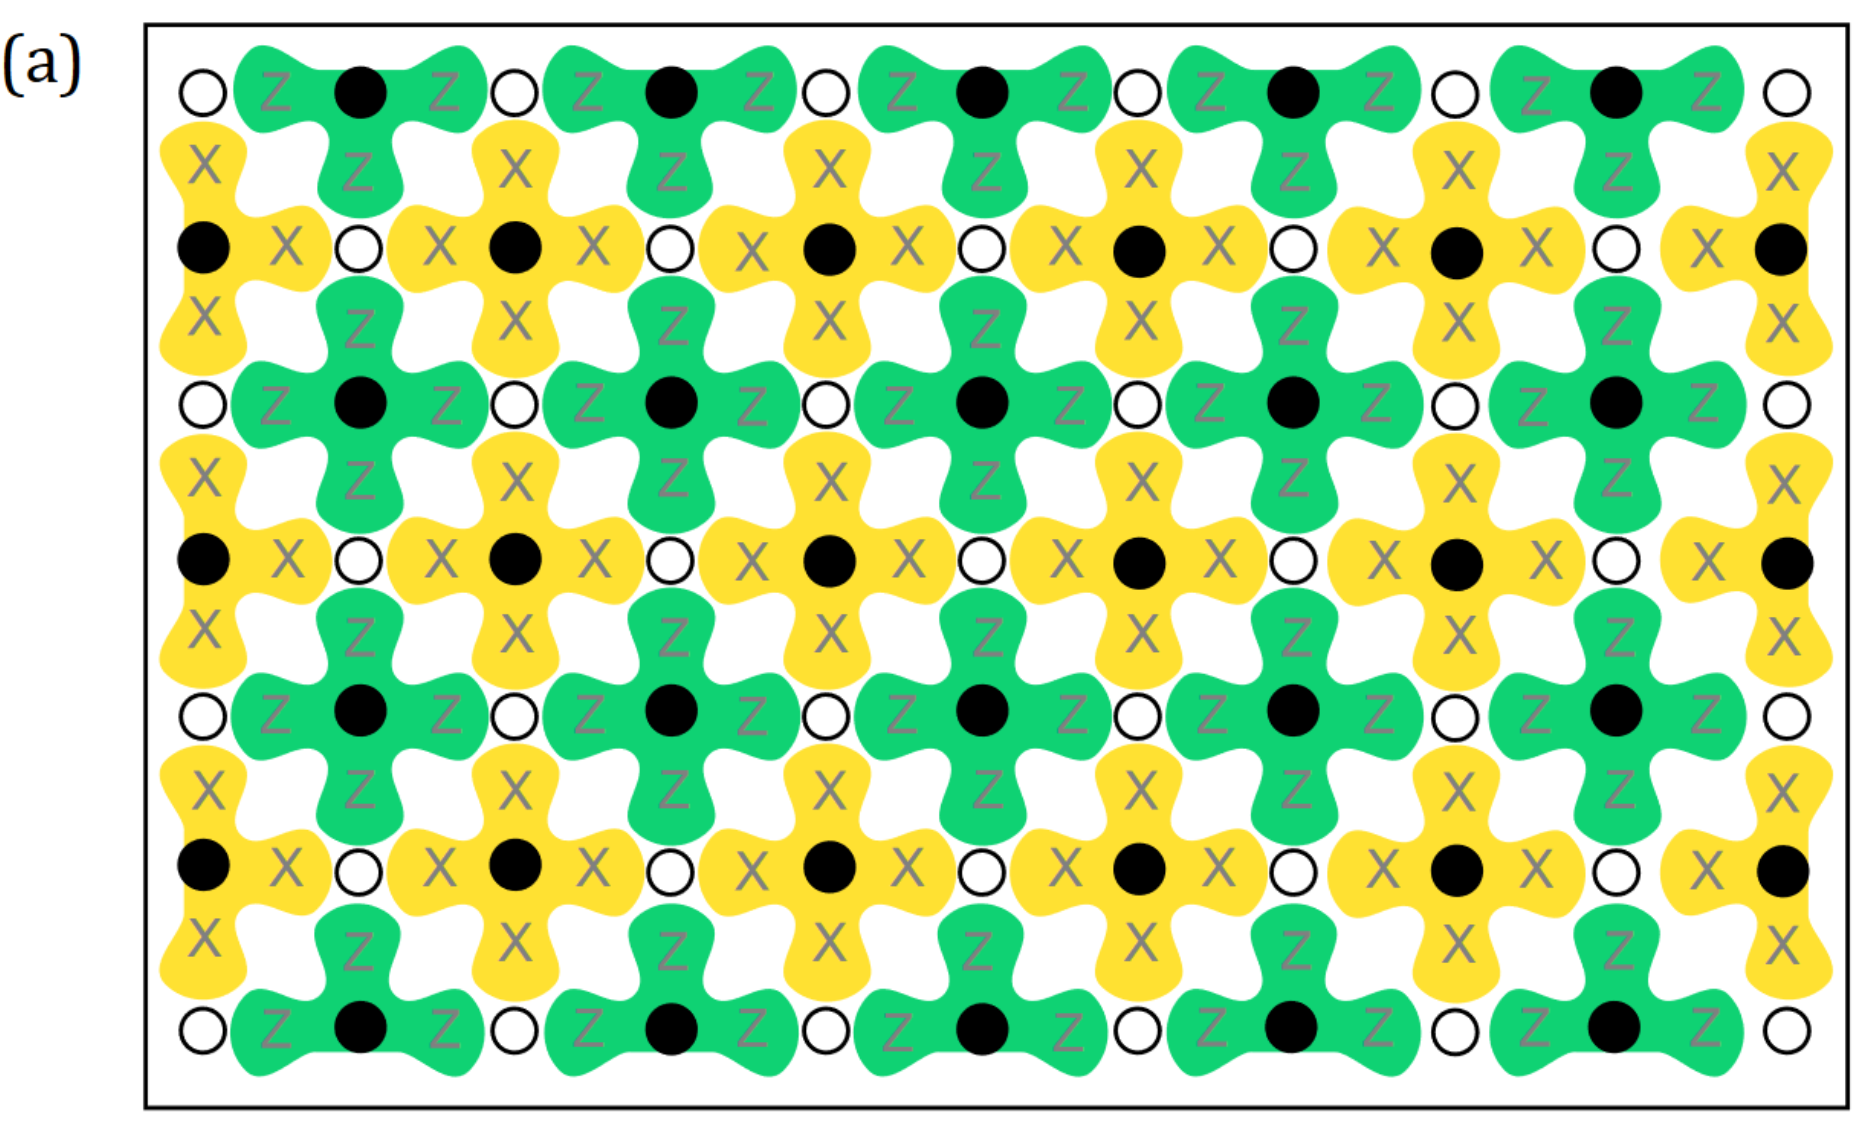
\includegraphics[width=8cm]{graphics/Introduction/surfacecode.PNG}
    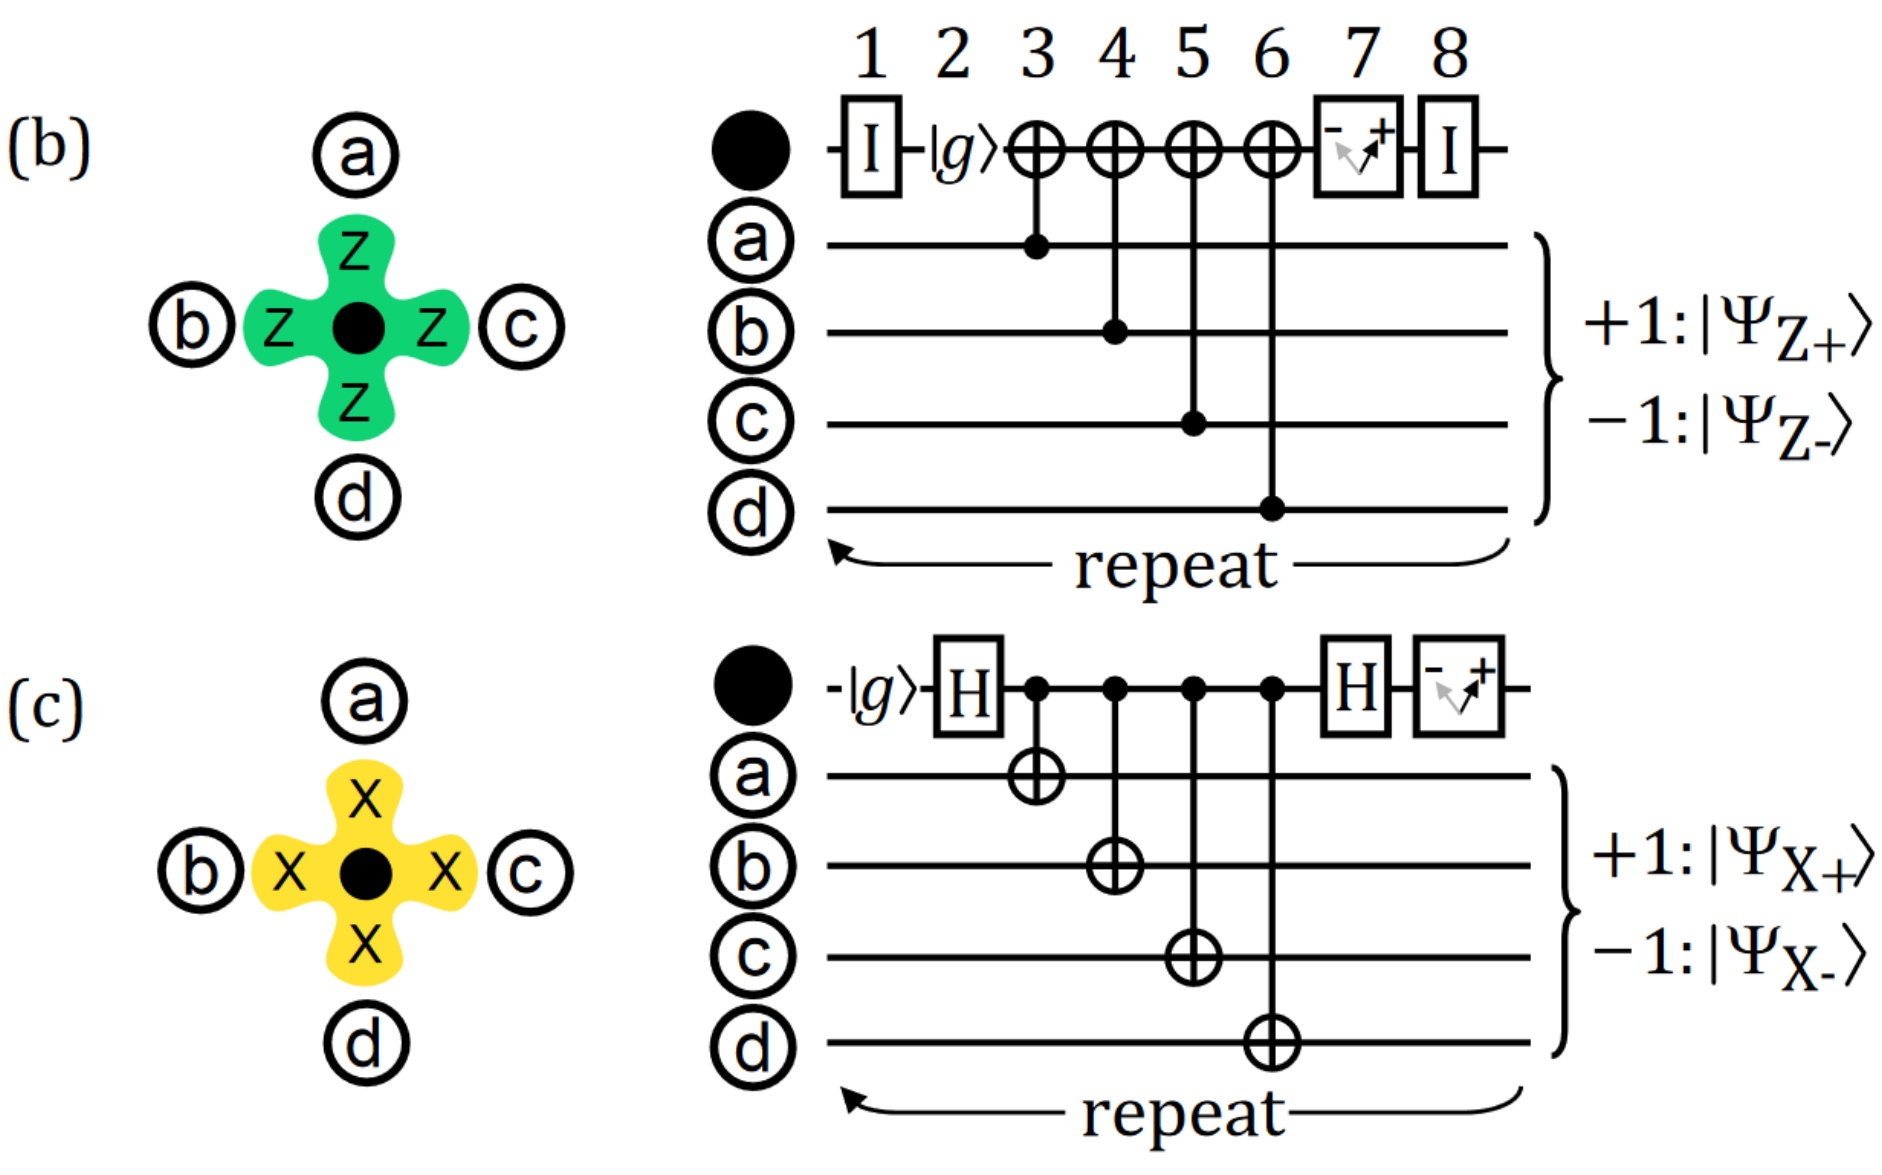
\includegraphics[width=8cm]{graphics/Introduction/surfacecode_stabilizers.PNG}
    \caption{Surface code layout and stabilizer measurements taken from Ref. \cite{fowler_surface_2012}. Left figure depicts physical layout of surface code, with white data qubits and black ancilla qubits alternating across the grid. Stabilizer routines on right show how correlations between groups of four data qubits are measured using ancilla qubits.}
    \label{fig:surface}
\end{figure}


\section{Silicon-based Quantum Computing}
Phosphorus donor nuclear and electrons spins are well understood 2-state quantum systems. When a phosphorus atom is implanted into silicon's tetrahedral crystal structure, four of its five electrons form covalent bonds with neighbouring silicon atoms, leaving one electron which is loosely bound, and spatially distributed over a large region\cite{kittel_introduction_2005}. This large spatial distribution facilitates interaction between the donor electrons of closely spaced phosphorus atoms, offering a means of interaction between qubits based on P donors in silicon. 

Silicon offers certain advantages over other materials which could be utilised for spin-based quantum computing, with low spin orbit coupling, and the capacity to be isotropically enriched to mitigate decoherence due to the nuclear spin bath. \cite{ager_high-purity_2005}. Silicon based devices are also at an advantage when it comes to scalability, being able to utilise the fabrication technologies which have been developed over the past several decades to fuel the rise of classical computers. 

In 1998, Bruce Kane proposed a quantum computing architecture based on the nuclear spins of single phosphorus donors in silicon, coupled together via a tunable exchange interaction between their loosely bound electrons.\cite{kane_silicon-based_1998}. In the same year, Loss and DiVincenzo published work detailing an architecture utising spins of lone electrons placed on quantum dots, and like the Kane proposal relied on tuning of the exchange interaction between these electrons\cite{loss_quantum_1998}.


The Hamilton of the nuclear-electron spin system is given by
\begin{align}
    H = \frac{\gamma_e}{2}B_Z \sigma_{z,e} - \frac{\gamma_P}{2}B_Z\sigma_{z,n} + A\bm{\sigma}_e\cdot\bm{\sigma}_n,
\end{align}
where $\gamma_e = 176$ G rad/s, $\gamma_P = 108$ rad/s are the gyromagnetic ratios of the electron and phosphorus nucleus respectively. The first two terms correspond to the Zeeman splitting due to a background $z$-directed magnetic field, $B_Z$. The last terms is the hyperfine interaction, which couples the nuclear and electron spins to one another. The background static field serves the purpose of splitting the energy levels of the spin-up and spin-down states of the nucleus and electron, as well as allowing the hyperfine term to be approximated as $A\bm{\sigma}_e\cdot\bm{\sigma}_n\approx A\sigma_{z,n}\sigma_{z,e}$




Since Kane's original proposal in 1998, silicon-based quantum computing has gained significant traction, with many milestones overcome which were initially thought impossible. Some achievements of the past decade include the implantation of single phosphorus atoms to $\pm 1$ lattice site precision\cite{sat}, electron spin coherence times exceeding seconds in isotropically purified silicon\cite{Electron-spin-coherence-exceeding-seconds}, high fidelity single shot spin readout\cite{single-shot}, demonstration of coherent manipulation of a single P donor qubit in silicon\cite{single-atom-electron-spin}, and successful entanglement of a pair of electron qubits via the exchange interaction\cite{he_two-qubit_2019}. 

Experiments on phosphorus donor qubits generally involve one or two P donor dots, with various gates positioned nearby which control the electropotential landscape. These gates are the tips of nanowires, and are implemented as highly P-doped regions of the silicon substrate. Single electron transistors are often present, which are needed for electron spin readout. Figure \ref{fig:sip-diagram} shows an STM picture of one of these setups.

\begin{figure}
    \centering
    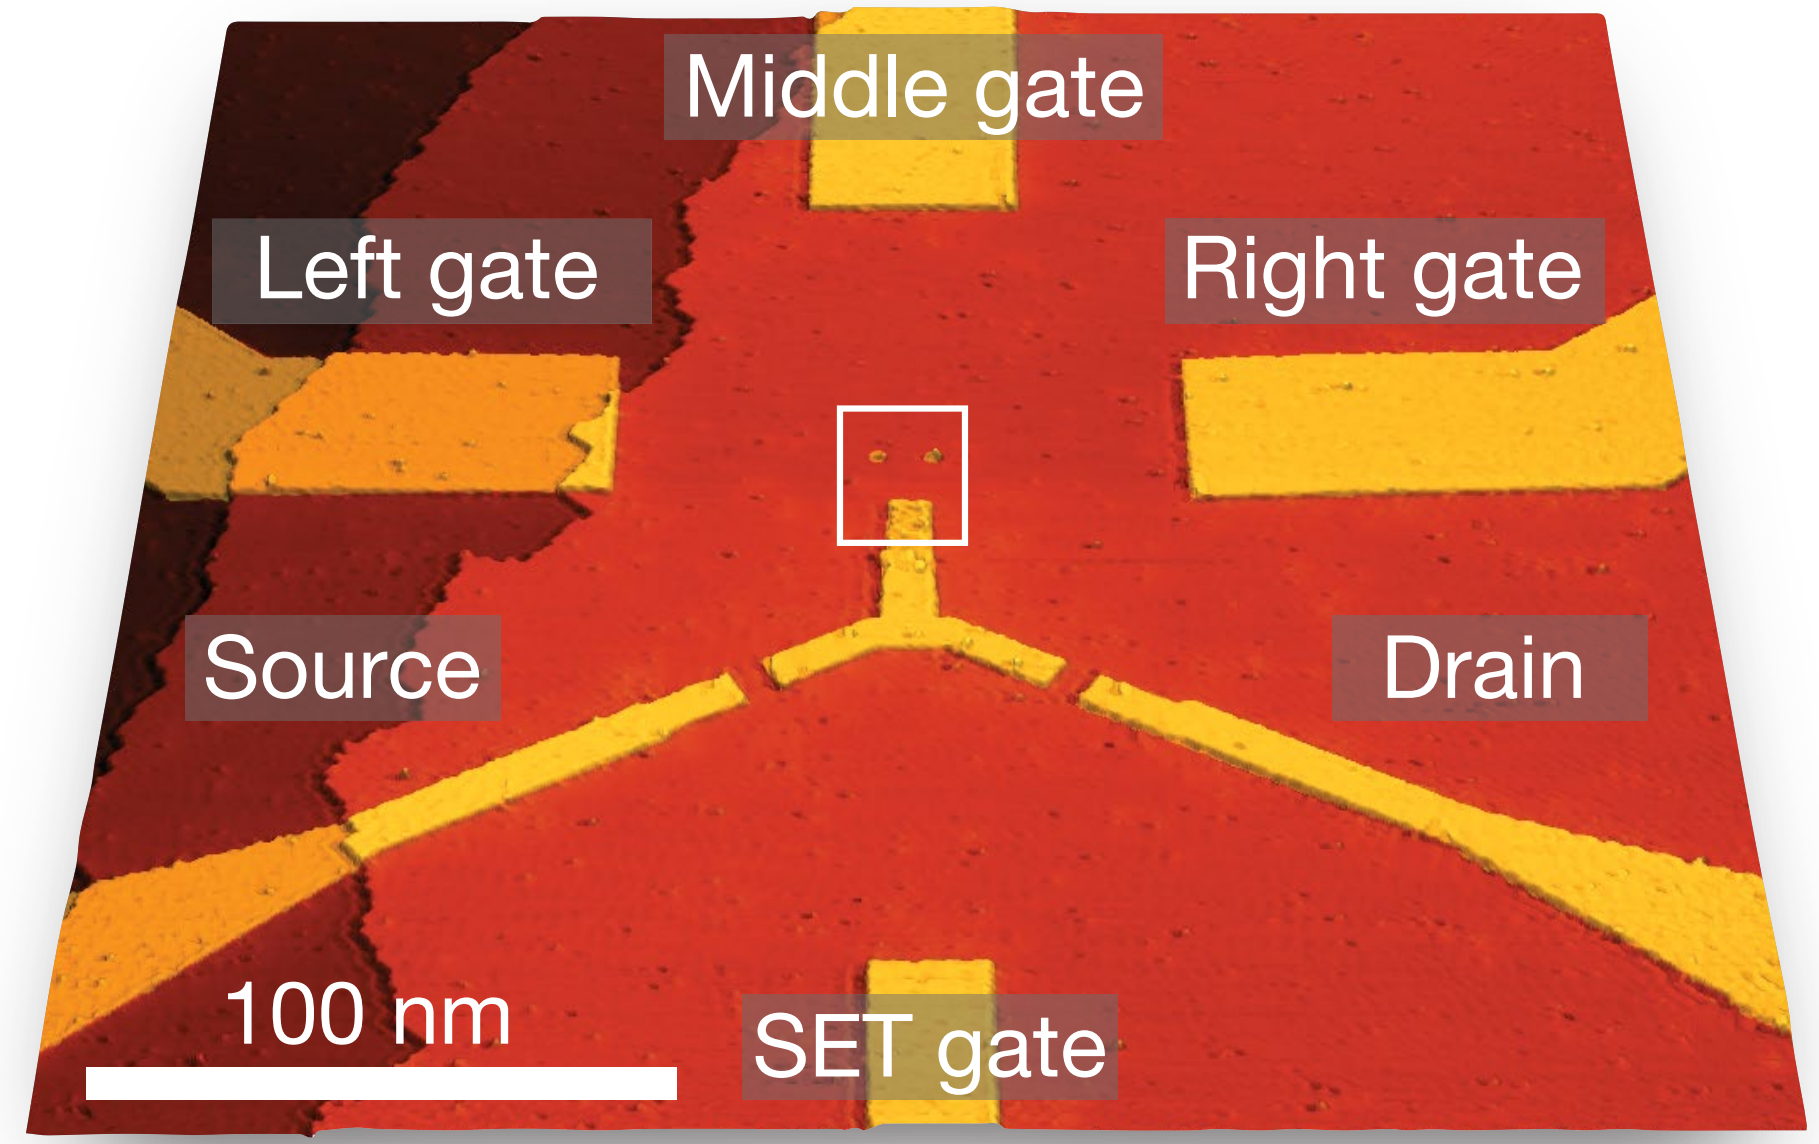
\includegraphics[width=8cm]{graphics/Introduction/swap_layout.PNG}
    \caption{Architecture used to demonstrate first $\sqrt{\text{SWAP}}$ gate between phosphorus donor electrons in silicon. Three-pronged SET island can can be seen between source and gate electrodes coming near enough to two quantum dots to facilitate electron tunneling.}
    \label{fig:swap-layout}
\end{figure}

Advances in fabrication technology now allow for placement of individual phosphorus with $\pm 1$ lattice site precision\cite{pla_single-atom_2012}. This utilises scanning tunneling microscopy (STM) hydrogen lithography techniques, a several step process. Saturation dosing of a three dimer patch with phosphene PH3 on the Si(100) surface at room temperature, resulting in adsorption of PH$_3$ molecules onto each dimer. Annealing at $350^\circ$, which facilitates dissociative processes\cite{wilson_thermal_2006}
\begin{align}
    PH_3\rightarrow PH_2+H\rightarrow PH_1+2H\rightarrow PH+3H,
\end{align}
and ultimately incorporation of a single $P$ atom into one of the 6 atomic sites of the three dimer patch. This method provides the level of precision required to create the arrays of single phophorus donors envisioned by Kane.

\subsection{Readout}
Readout of silicon based spin qubits requires a single electron transistor (SET) to be positioned close enough to the QD to facilitate electron tunneling between the QD and SET island. SETs are nano-scale electronic devices consisting of source and drain electrodes coupled to a conducting island via tunnel junctions. These are patterned in the silicon substrate as regions of high doping concentration. The source-drain tunnel current can be turned on or off by by a change in the charge content near the SET island, due to the Coulomb blockade effect. The behaviour of SETs and Coulomb blockade is outlined in more detail in figure \ref{fig:coulomb-blockade}.

\begin{figure}
    \centering
    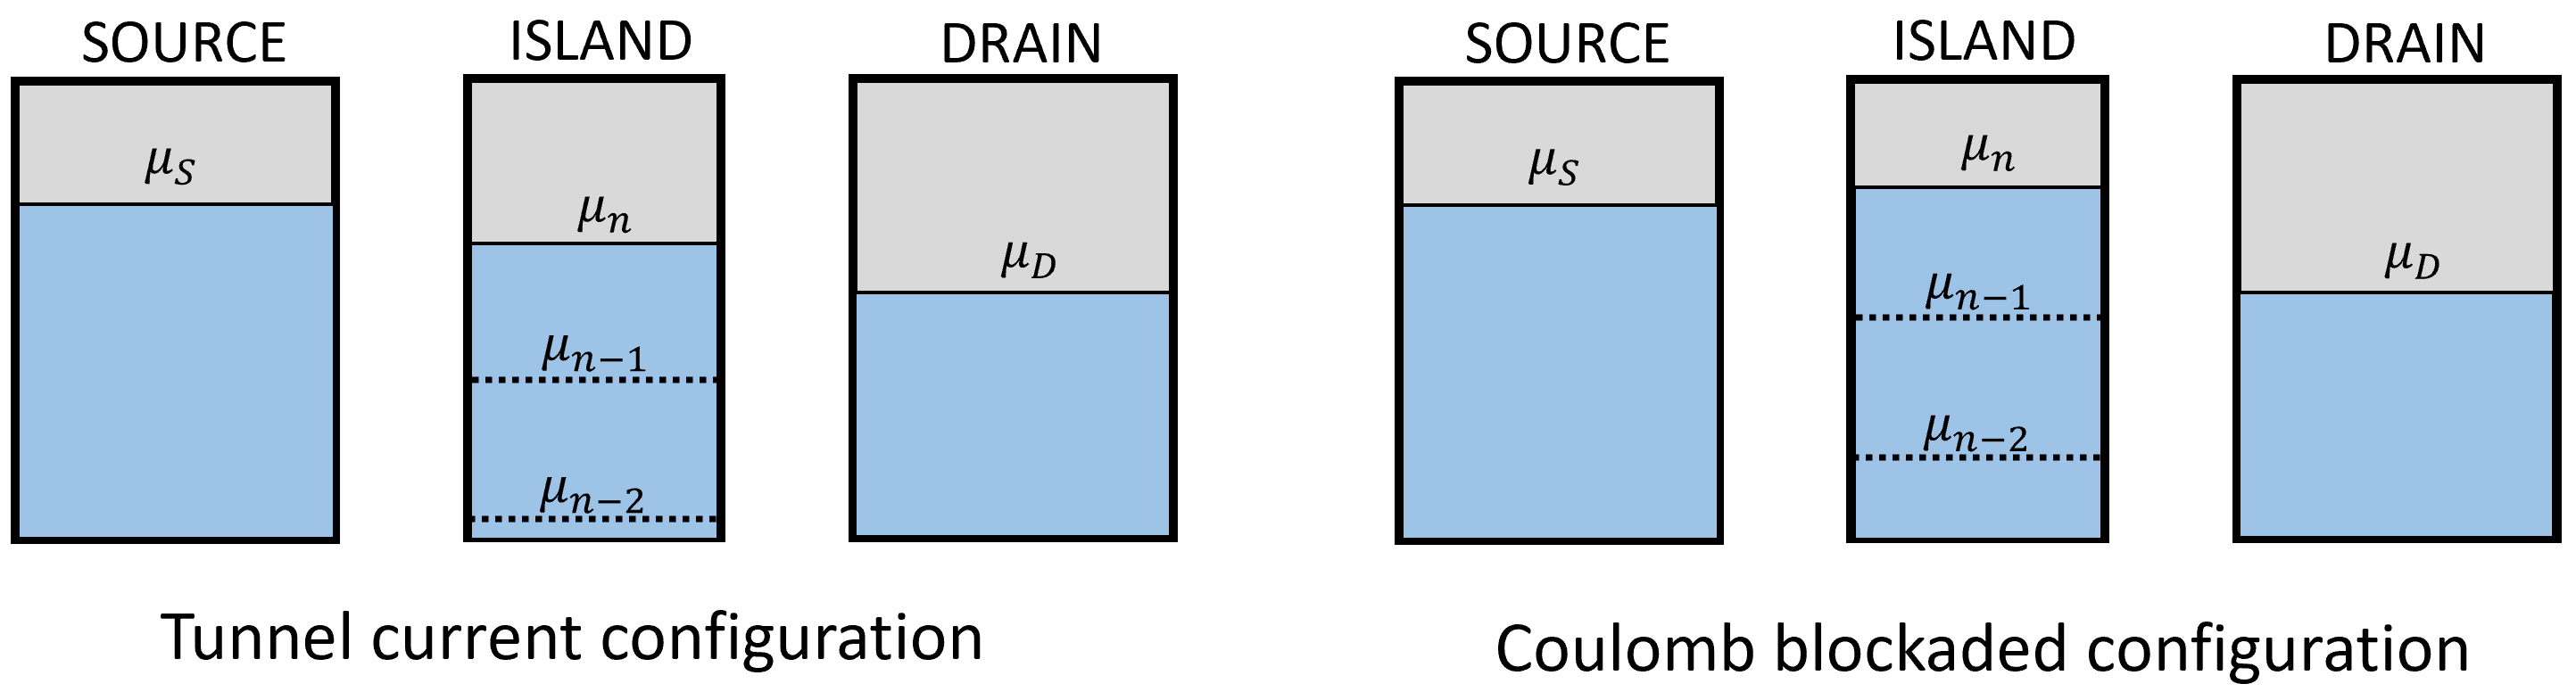
\includegraphics[width=14cm]{graphics/Introduction/coulomb_blockade.PNG}
    \caption{Fermi levels of source, island, and drain of single electron transistor. Configuration on the left allows current electrons to flow from source to drain, as tunneling through each barrier constitutes a step down in energy, and is thus favourable. Coulomb blockade is shown in the right configuration, where current is unable to flow even though the source Fermi level is higher than the drain. This is because the highest energy electron on the island experiences Fermi level $\mu_{n-1}$, with its own charge not contributing, making it unfavourable to tunnel to the drain. Note that Coulomb blockade can be entered by changing only the island Fermi level (as shown above). The presence of charge in the vicinity of, but external to, the SET island, can cause this shift in Fermi level, thus shutting off the current and achieving transistor-like behaviour.}
    \label{fig:coulomb-blockade}
\end{figure}

Electron spin readout relies on spin-dependent tunneling of electrons from the P donor to a nearby single electron transistor (SET) island\footnote{Nuclear spin readout requires swapping of nuclear and electron spins followed by electron spin readout}. This is possible due to Zeeman splitting of the electron spin states under the influence of the large background static magnetic field, $B_Z$. The source and drain leads can be used to tune the SET island Fermi level such that it lies between the Fermi levels of the spin-up and spin-down states of the electron, as shown in figure \ref{fig:readout-levels}. If a spin-up electron is present, a tunneling event occurs. The electron tunnels from the donor to the SET island and straight out via the drain. This can be designed such that the change in charge content in the vicinity of the SET island then lifts the SET out of Coulomb blockade, resulting in a sudden current through the source and drain leads, which indicates readout of the spin-up state.

\begin{figure}
    \centering
    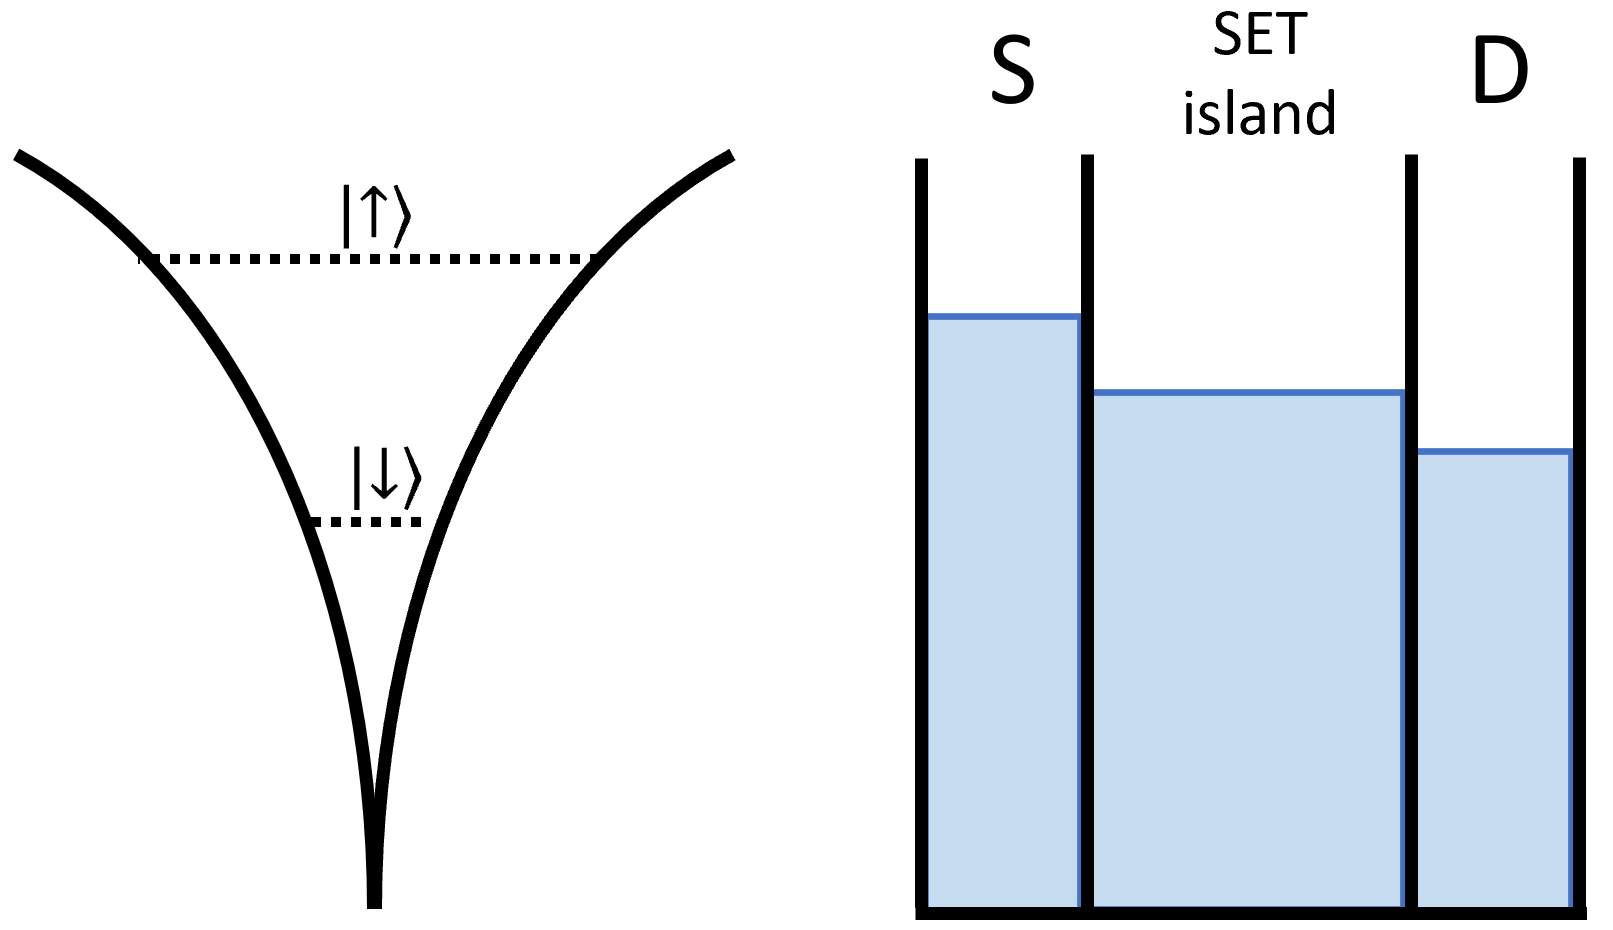
\includegraphics[width=8cm]{graphics/Introduction/readout_levels.PNG}
    \caption{Energies of the spin states of an electron residing on a donor, with nearby SET island tuned such that its Fermi level lies directly in between the two donor electron energies, permitting only an electron in the spin-up state to tunnel out.}
    \label{fig:readout-levels}
\end{figure}

The electron spin measurement regime described above is based on a 2010 publication by researchers at UNSW, in which they demonstrate successful single-shot readout of P donor electron spins in silicon\cite{morello_single-shot_2010}. A modified version of this procedure was then demonstrated in 2013\cite{pla_high-fidelity_2013}, where spin of the donor electron determines whether or not a second electron can tunnel onto the donor. When the donor electron is in the higher energy spin-up state, less energy is required to reach the two-electron ground state, thus allowing for spin dependent tunneling from SET to donor. The SET, donor energy levels and characteristic source-drain current pulses for each regime are shown in figure \ref{fig:readout}. 
\begin{figure}
    \centering
    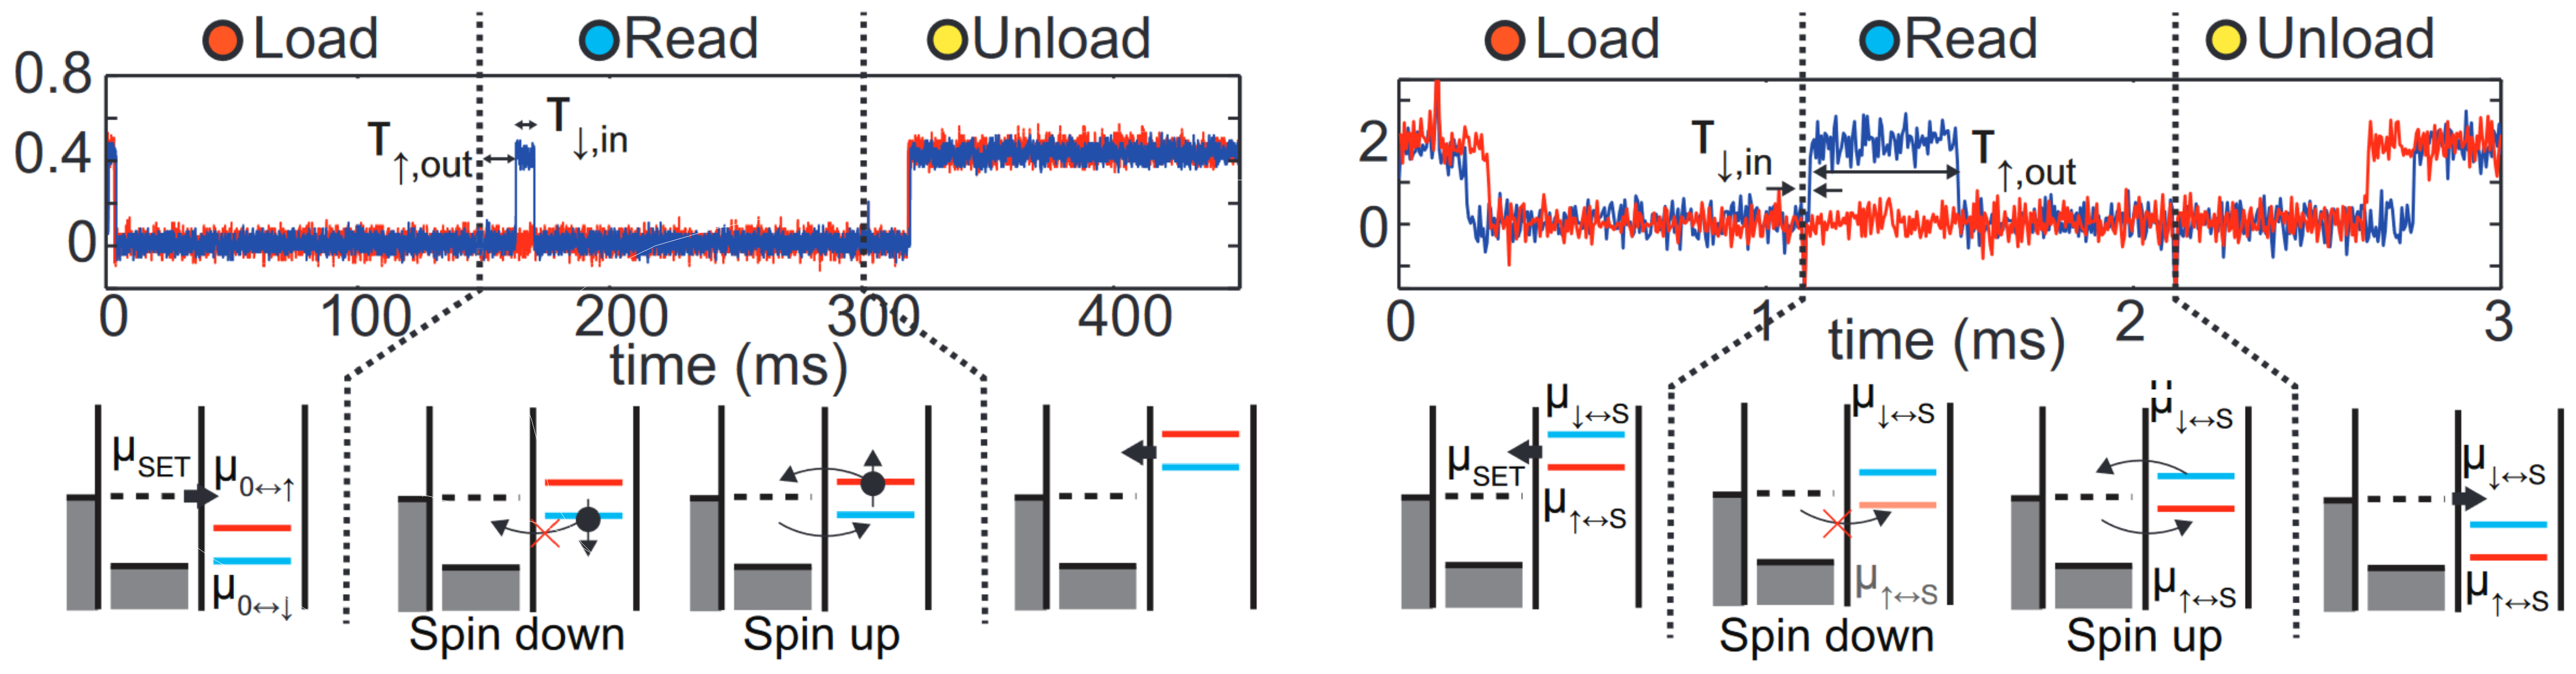
\includegraphics[width=16cm]{graphics/Introduction/readout_AB.PNG}
    \caption{Caption}
    \label{fig:readout}
\end{figure}

\subsection{The exchange interaction}
Gates between neighbouring pairs of qubits are carried out via the exchange interaction. The exchange interaction describes a splitting in energy between the states of two-electron systems which occurs due to the Pauli exclusion principle\cite{kittel_introduction_2005}.

The exchange interaction between the donor electrons of phosphorus dopants in silicon as a function of donor separation has been studied extensively, with various approaches taken to calculating exchange coupling strength, including hydrogenic\cite{fang_effects_2002},
effective mass\cite{koiller_exchange_2001,wellard_voltage_2004}, and 
tight binding \cite{wang_highly_2016} approximations.
 
Exchange interaction strength proves to be extremely sensitive to slightly changes in donor separation, or electric field. This posese a challenge for gates designed based on exchange, with the $\pm 1$ lattice site previously mentioned resulting in vastly different exchange strengths, and low levels of electric field noise liable to disrupt gate operation.
 
The exchange interaction is described by the Heisenberg Hamiltonian,
\begin{align} 
H = J\bm{\sigma}\cdot\bm{\sigma},
\end{align}
which describes an energy splitting of $4J$ between singlet and triplet states 
\begin{align}
    \ket{S} &= \frac{1}{\sqrt{2}}(\ket{01}-\ket{10}),\\[4pt]
    \ket{T_+}&=\ket{000}\\
    \ket{T_0} &= \frac{1}{\sqrt{2}}(\ket{01}+\ket{10})\\
    \ket{T_-} &= \ket{111}
\end{align}



\section{Quantum control}
Physical implementation of quantum computing gates is carried out via application of carefully designed magnetic field pulses. These pulses are tuned to be able to excite the desired transition within the quantum system which corresponds to a given gate. Principles of quantum control can be harnessed to numerically design pulses which achieve a target unitary on a particular quantum system. Quantum control applies principles of optimal control to quantum mechanical systems, and has been widely applied to magnetic resonance\cite{conolly_optimal_1986}.

Optimal control is a powerful tool in which physical problems characterised by a path through some parameter space are optimised through the minimisation of a cost function which depends on this path. Optimal control has a rich history in physics, with early examples including Fermat's principle, where the cost function is the time taken by light to pass through a series of media, or the Principle of Least Action, whose cost function is the action\cite{sargent_optimal_2000}. Interest in quantum control has piqued far more recently, however, with the proliferation of the computer making powerful numerical approaches far more tenable than before. 



One such numerical approach is gradient ascent pulse engineeing, or GRAPE, which can be used to design magnetic field pulses to produce a desired unitary for a given quantum system\cite{khaneja_optimal_2005,rowland_implementing_2012}. In general, a quantum system described by some Hamiltonian $H_0$ will naturally oscillate with certain frequencies, called resonant frequencies. Application of control fields, denoted $H_k$, which oscillate at these resonant frequencies, are able to excite transitions of the system between its different states. 

GRAPE has previously been used to determine optimal pulses for transitions in spin qubit systems based on silicon phosphorus\cite{hill_exchange-based_2021}, as well as nitrogen-vacancy (NV) centres in diamond\cite{rong_experimental_2015}. GRAPE can also be used to optimise hyperfine and exchange coupling strengths over the duration of a gate if precise control over these parameters is assumed\cite{tsai_optimal_2009}.

Following the approach of Khaneja et. al., with the Hamiltonian of a  system can be expressed as
\begin{equation}
    H = H_0 + \sum_{k=1}^m u_k(t)H_k(t).
    \label{eq:ham-cont}
\end{equation}
The control vectors $u_k(t)$ serve to modulate the amplitudes of each applied control field. These are the parameters which are to be optimised via gradient descent. 



Equation \ref{eq:ham-cont} is discretised into $N$ timesteps each having length $\delta t$, so as to be suitable for solving computationally. 
\begin{equation}
    H = H_0 + \sum_{k=1}^m u_{kj}H_{kj}
    \label{eq:ham-disc}
\end{equation}
We can determine time evolution resulting from application of Hamiltonian \ref{eq:ham-disc} by first calculating sub-operators for each time step,
\begin{equation}
    U_j = \exp\left\{-i\left(H_0 + \sum_{k=1}^m u_{kj}H_{kj}\right)\right\},
\end{equation}
and then combining,
\begin{equation}
    U_f = U_{N-1}\dots U_0.
\end{equation}
This is then compared with the desired target unitary, $U_t$, with the fidelity calculated as
\begin{equation}
    \Phi = \bra{U_t}\ket{U_f}\bra{U_f}\ket{U_t}
\end{equation}
where 
\begin{equation}
    \bra{A}\ket{B} = \frac{1}{d}\Tr\left(A^\dagger B\right)
\end{equation}
is the standard inner product of $d$-dimensional square matrices.

We now have a means of finding optimal pulses to design target unitaries. One can program a cost function which takes control parameters $u_{kj}$ as input, and outputs cost $J=1-\Phi$,\footnote{Conventional optimisers usually perform minimisation rather than maximisation, so we define a cost function whose minimisation will maximise our fidelity, the most natural option being $J=1-\Phi$.} and pass this to an optimiser. 

Khaneja et. al.'s was influential because it took this a step further, providing a method by which to calculate the gradient of the fidelity analytically, thereby providing an enormous speed up to the optimisation.

The forward propagated time-evolution operator and back propagated target are stored for each step, defined by
\begin{equation}
    X_j = U_jU_{j-1} \dots U_1,\quad P_j = U_{j+1}^\dagger U_{j+2}^\dagger\dots U_N^\dagger
\end{equation}
It can be observed that 
\begin{equation}
    \bra{U_f}\ket{U_t} = \bra{X_j}\ket{X_j} = \bra{U_j X_{j-1}}\ket{P_j},
\end{equation}
which gives
\begin{align}
    \frac{\partial\Phi}{\partial u_{kj}} &= \frac{\partial}{\partial u_{kj}} \bra{P_j}\ket{U_jX_{j-1}}\bra{U_jX_{j-1}}\ket{P_j}\\
    &= \left\langle P_j\left|\frac{\partial U_j}{\partial u_{kj}}\right. X_{j-1}\right\rangle\bra{X_j}\ket{P_j} + \text{c.c.}
\end{align}
The first order approximation $\frac{\partial U_j}{\partial u_{kj}} = -i\delta t H_{kj}U_j$ then gives
\begin{equation}
      \frac{\partial\Phi}{\partial u_{kj}} = -2\text{Re}\langle P_j | i\delta tH_{kj} X_j\rangle \langle X_j | P_j\rangle
\end{equation}





\end{document}